\documentclass[]{beamer}
\usepackage[german]{babel}
\usepackage[latin1]{inputenc}
\usepackage[T1]{fontenc}
\usepackage{ae}
\usepackage{amsmath}  		  % f�r erw. Formeloptionen, Option [] zur Vermeidung von Type3-Fonts
\usepackage{amstext}          % f�r Klartext via \text{} in Formeln
\usepackage{amsfonts}         % f�r komplexere Formeln (Mengensymbole ...)
\usepackage{amssymb}          % f�r komplexere Formeln (Mengensymbole ...)
\usepackage{graphicx} 		  % Einbindung von Grafiken (pdf, png, jpg)
\usepackage{dsfont}
\usepackage{bm} 
\usepackage{mathrsfs}
\usepackage{setspace}
\usepackage{enumerate}        % verbessert Aufz�hlungen
\usepackage{array}            % f�r Tabellen: bindet tabular-Umgebung ein
\usepackage{multicol}         % zur Indexerstellung in zwei Spalten
\usepackage{amsthm}
\usepackage{tabularx}
\usepackage{longtable}
\usepackage{adjustbox}
\usepackage{rotating}


% Theme %
\usetheme{CambridgeUS}

\definecolor{redbrown}{RGB}{175,0,0}
\definecolor{alert}{RGB}{200,0,0}
\definecolor{lightgray}{RGB}{4,6,76}
\definecolor{white}{RGB}{255,255,255}
\definecolor{green1}{RGB}{0,126,0}


% rahmenfarbe %
\setbeamercolor{block title}{fg=white,bg=redbrown}
\setbeamercolor{block title alerted}{use=alerted text,bg=alerted text.fg!75!bg}
\setbeamercolor{block title example}{use=example text,bg=example text.fg!75!bg}

% blockfarbe %
\setbeamercolor{block body}{parent=normal text,use=block title,bg=block title.fg!92!fg}
\setbeamercolor{block body alerted}{parent=normal text,use=block title alerted,bg=block title alerted.bg!25!bg}
\setbeamercolor{block body example}{parent=normal text,use=block title example,bg=block title example.bg!25!bg}
\setbeamercolor{bgcolor}{parent=normal text,use=block title,bg=block title.fg!92!fg}


% zeilenabstand zwischen itemizeobjekten %

\makeatletter
\renewcommand{\itemize}[1][]{%
\beamer@ifempty{#1}{}{\def\beamer@defaultospec{#1} }%
\ifnum \@itemdepth >2\relax\@toodeep\else
\advance\@itemdepth\@ne
\beamer@computepref\@itemdepth% sets \beameritemnestingprefix
\usebeamerfont{itemize/enumerate \beameritemnestingprefix body}%
\usebeamercolor[fg]{itemize/enumerate \beameritemnestingprefix body}%
\usebeamertemplate{itemize/enumerate \beameritemnestingprefix body
begin}%
\list
{\usebeamertemplate{itemize \beameritemnestingprefix item}}
{\setlength\itemsep{15pt}%%%%%%%%%%%%%%% %%%%%%%%%%%%%%%
\def\makelabel##1{{\hss\llap{{%
\usebeamerfont*{itemize \beameritemnestingprefix item}%
\usebeamercolor[fg]{itemize \beameritemnestingprefix 
item}##1}}%
}}}
\fi%
}

\setbeamertemplate{enumerate item}
{
  \begin{pgfpicture}{-1ex}{-0.65ex}{1ex}{1ex}
    \usebeamercolor[fg]{item projected}
    {\pgftransformscale{2}\pgftext{\Large\pgfuseshading{bigsphere}}}
    {\pgftransformshift{\pgfpoint{0pt}{0.5pt}}
      \pgftext{\usebeamerfont*{item projected}\footnotesize\insertenumlabel}}
  \end{pgfpicture}%
}

\renewcommand*{\footnoterule}{ \hrule \@width 2in \kern 2.6pt}

\makeatother

% praesentationsbeginn %

\begin{document}

\beamertemplatenavigationsymbolsempty

\title[EvoAlg]{Evolution�re Algorithmen zur Minimierung der Griewank-Funktion}   
\author[D. Gilgen, J.Zschoche]{Daniel Gilgen, Jan Zschoche}
\institute[BA Leipzig]{
Berufsakademie Leipzig
} 
\date[Leipzig, 2016]{}

\begin{frame}
    \titlepage
\end{frame}

\begin{frame}\frametitle{Gliederung}
    \vspace{1cm}
    \begin{enumerate}
	\item \textbf{\large Einleitung}\\
		Aufbau eines evolution�ren Algorithmus, Strategie- und Parameterwahl, Auswertung \\[0.4cm]
	\item \textbf{\large Ergebnisse f�r konstante Mutationsrate}\\[0.4cm]
	\item \textbf{\large Ergebnisse f�r mit Alter wachsender Mutationsrate}\\[0.4cm]
	\item \textbf{\large Ergebnisse f�r mit Alter abnehmender Mutationsrate}\\
    \end{enumerate}
\end{frame}

%%%%%%%%%%%%%%%%%%%%%%%%%%%%%%%%%%%%%%%%%%%%%%%%%%%%%
%			Einleitung		    %
%%%%%%%%%%%%%%%%%%%%%%%%%%%%%%%%%%%%%%%%%%%%%%%%%%%%%

\section{Einleitung} 

% Framebeginn...%
\begin{frame}\frametitle{Einleitung} 
	
	\begin{center}
		\LARGE{Einleitung}	
	\end{center}
	
\end{frame}

% Framebeginn...%
\begin{frame}\frametitle{Aufbau des verwendeten EvoAlg} 

	\hspace{-0.25cm}
	\begin{picture}(0,150)%
		\only<1->{\put(0,0){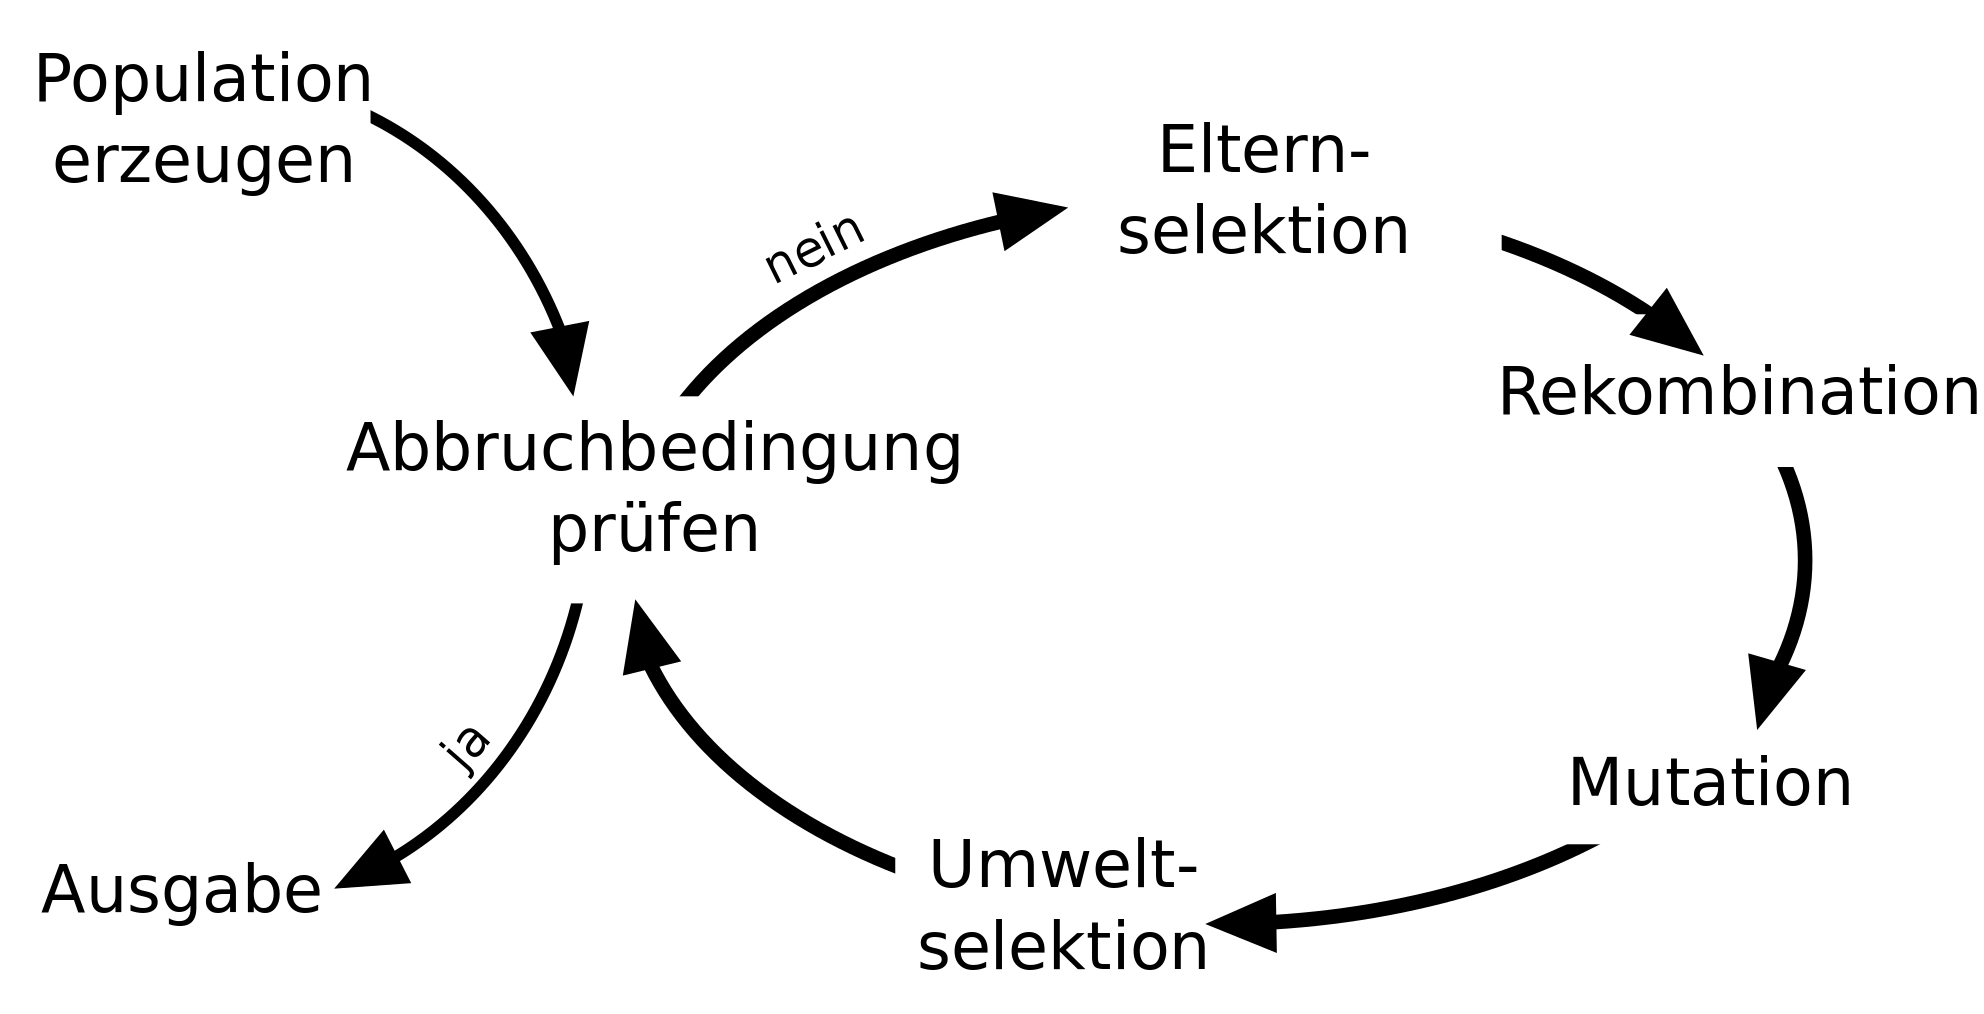
\includegraphics[width=0.9\linewidth]{abbildungen/algorithm.png}}}%
		\only<2->{\put(130,75){\color{alert}\parbox{4cm}{%
		    \begin{align*} 
			F^\text{min} & < 10^{-4} \\[-0.2cm]
			 \sigma_{F}  & < 10^{-4} \\[-0.1cm]
			   gen 	     & > 3000
		    \end{align*}}
		}}
		\only<3-6>{\put(200, 155){\color{alert}\parbox{4cm}{zufallsbasiert,\newline rangbasiert}}}%
		\only<4->{\put(280, 110){\color{alert}\parbox{4cm}{intermedi�r}}}%
		\only<5-6>{\put(260, 10){\color{alert}\parbox{4cm}{zeitlich konstant,\newline altersabh�ngig}}}%
		\only<6->{\put(165, -17){\color{alert}\parbox{4cm}{50\% zufallsbasiert,\newline 50\% rangbasiert}}}%
		\only<7>{\put(200, 155){\color{alert}\parbox{4cm}{ \large \textbf{zufallsbasiert,}\newline \textbf{rangbasiert}}}}
		\only<7>{\put(260, 10){\color{alert}\parbox{4cm}{\large \textbf{zeitlich konstant,}\newline \textbf{altersabh�ngig}}}}

	\end{picture}%

\end{frame}

% Framebeginn...%
\begin{frame}\frametitle{Elternselektion detailiert} 

	\begin{picture}(0,140)%
	\only<1>{\put(60,0){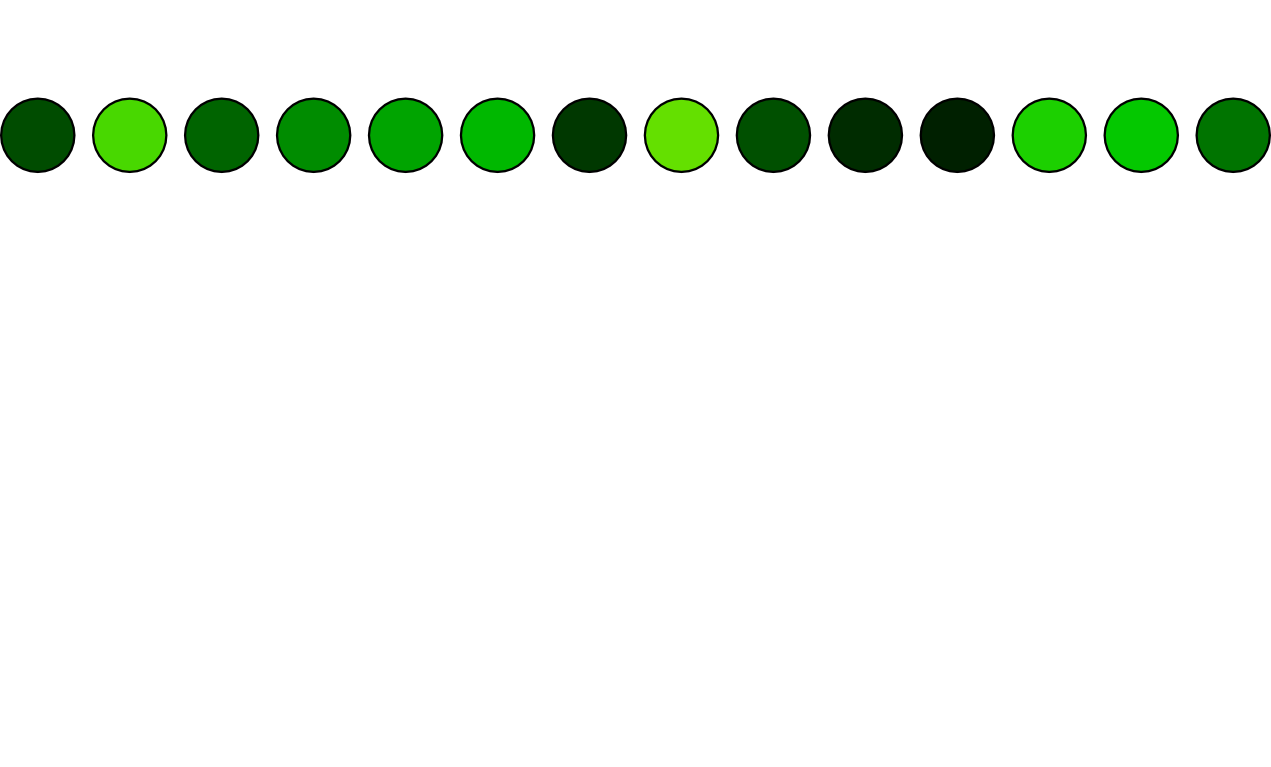
\includegraphics[width=0.7\linewidth]{abbildungen/detParSel0.png}}}%	
	\only<2>{\put(60,0){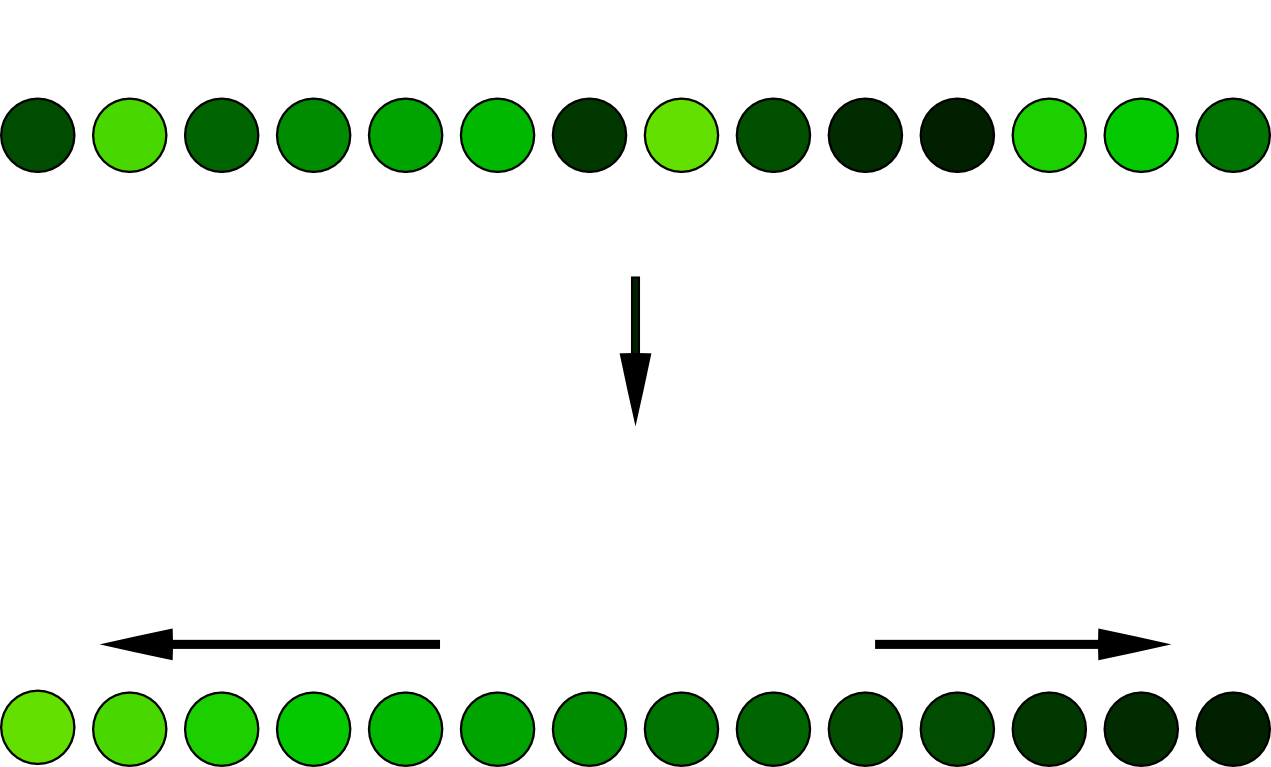
\includegraphics[width=0.7\linewidth]{abbildungen/detParSel1.png}}}%	
	
	\only<3>{\put(60,0){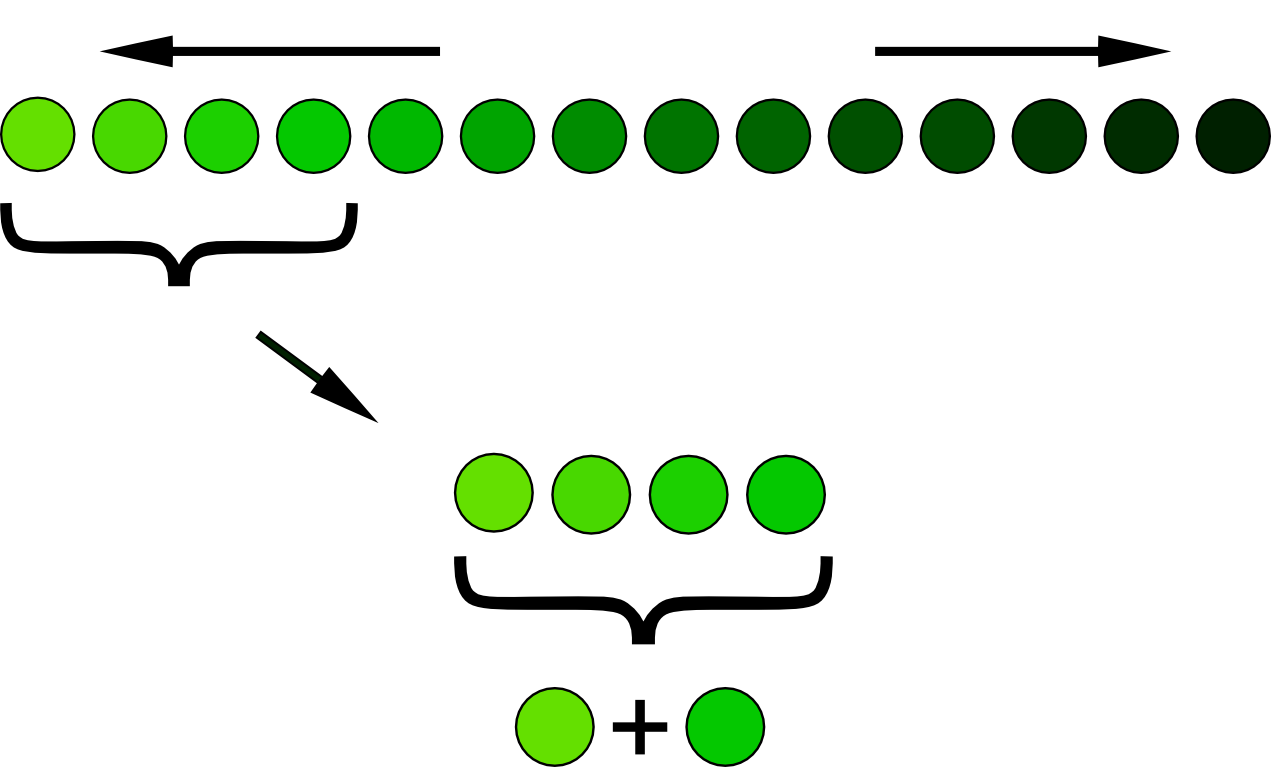
\includegraphics[width=0.7\linewidth]{abbildungen/detParSel2.png}}}%	
	
	\only<1->{\put(0,160){\parbox{8cm}{\Large \textbf{Rangbasierte Selektion:}}}}%
	\only<1-2>{\put(160, 135){\parbox{4cm}{\textbf{unsortiert}}}}%
	\only<2>{\put(165, 20){\parbox{4cm}{\textbf{Fitness}}}}%
	\only<2>{\put(70, 30){\parbox{4cm}{besser}}}%
	\only<2>{\put(250, 30){\parbox{4cm}{schlechter}}}%
	\only<3>{\put(165, 135){\parbox{4cm}{\textbf{Fitness}}}}%
	\only<3>{\put(70, 142){\parbox{4cm}{besser}}}%
	\only<3>{\put(250, 142){\parbox{4cm}{schlechter}}}%
	\only<3>{\put(230, 45){\parbox{4cm}{\textbf{Gruppe der\newline Besten}}}}%
	\only<3>{\put(230, 5){\parbox{4cm}{\textbf{Zufallsauswahl}}}}%
	\end{picture}%

\end{frame}

% Framebeginn...%
\begin{frame}\frametitle{Zwischenstand} 

	\hspace{-0.25cm}
	\begin{picture}(0,150)%
		\put(0,0){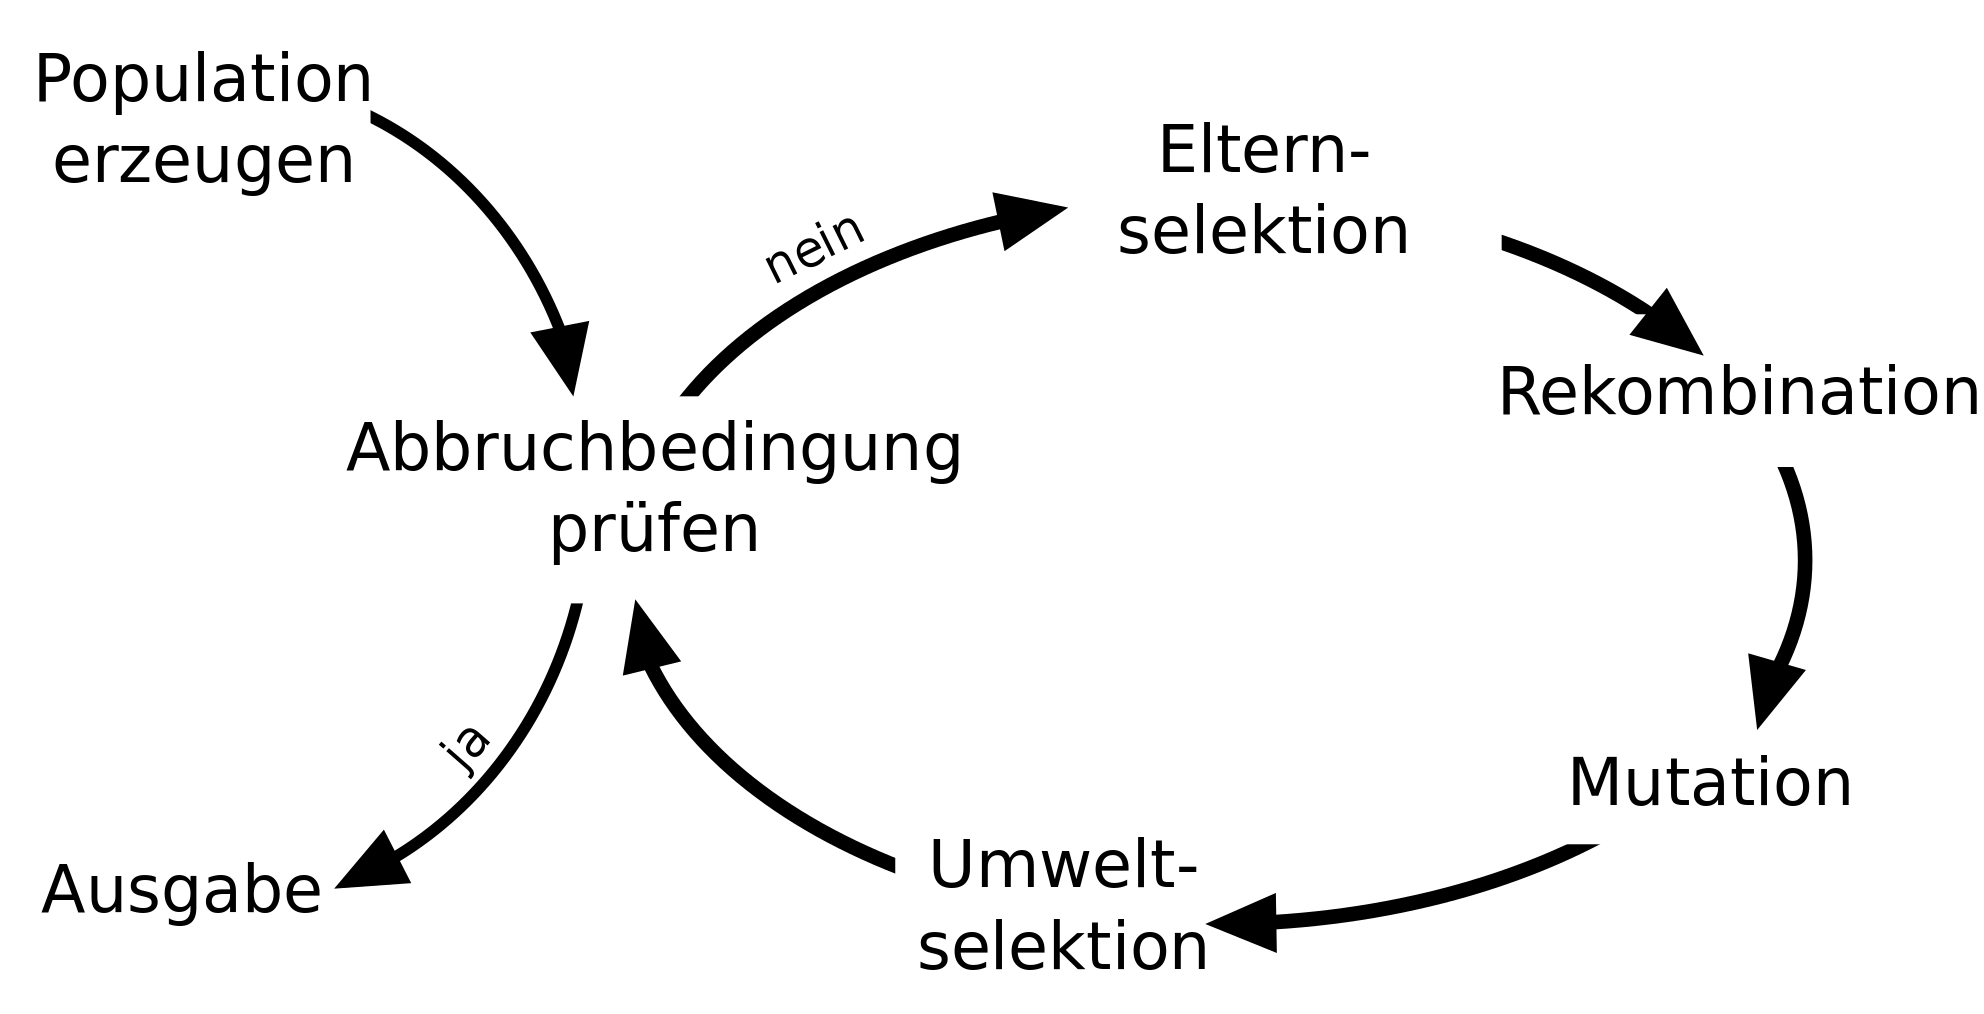
\includegraphics[width=0.9\linewidth]{abbildungen/algorithm.png}}%
		\put(280,150){
\includegraphics[width=0.08\linewidth]{abbildungen/Yes_check.png}}%
		\put(130,75){\color{alert}\parbox{4cm}{%
		    \begin{align*} 
				F^\text{min} & < 10^{-4} \\[-0.2cm]
				 \sigma_{F}  & < 10^{-4} \\[-0.1cm]
				   gen 	     & > 3000
		    \end{align*}}
		}
		\put(280, 110){\color{alert}\parbox{4cm}{intermedi�r}}%
		\put(165, -17){\color{alert}\parbox{4cm}{50\% zufallsbasiert,\newline 50\% rangbasiert}}%
		\put(200, 155){\color{alert}\parbox{4cm}{ \large \textbf{zufallsbasiert,}\newline \textbf{rangbasiert}}}
		\put(260, 10){\color{alert}\parbox{4cm}{\large \textbf{zeitlich konstant,}\newline \textbf{altersabh�ngig}}}

	\end{picture}%

\end{frame}

% Framebeginn...%
\begin{frame}\frametitle{Mutation -- detailiert I} 

	\begin{minipage}[t]{0.5\linewidth}
	    \begin{picture}(0,0)%

		\only<1->{
		    \put(20,50){
\includegraphics[width=0.7\linewidth]{abbildungen/Genom1.png}}%
		    \put(0,80){\parbox{4cm}{\Large \textbf{Genom:}}}%
		    \put(26,55){\parbox{4cm}{$g_{1}$}}%
		    \put(45,55){\parbox{4cm}{$g_{2}$}}%
		    \put(65,55){\parbox{4cm}{$g_{3}$}}%
		    \put(85,55){\parbox{4cm}{$g_{4}$}}%
		    \put(105,55){\parbox{4cm}{$g_{5}$}}%
		    \put(125,55){\parbox{4cm}{$g_{6}$}}%


		    \put(29,2){
\includegraphics[height=1.5cm]{abbildungen/arrow.png}}%

		    \put(10, 23){\parbox{6cm}{%
			\begin{align*}%
			    \tilde{g}_{1}\! = & \; rnd()\! <\! m(a)\, ? \\ 
					       & \;(g_{1}\! +\! M_\text{rnd})\, :\, g_{1};
			\end{align*}}}%
		}
		\only<1>{
		    \put(20,-20){
\includegraphics[width=0.7\linewidth]{abbildungen/Genom.png}}%
		    \put(26,-15){\parbox{4cm}{$\tilde{g}_{1}$}}%
		    \put(45,-15){\parbox{4cm}{$g_{2}$}}%
		    \put(65,-15){\parbox{4cm}{$g_{3}$}}%
		    \put(85,-15){\parbox{4cm}{$g_{4}$}}%
		    \put(105,-15){\parbox{4cm}{$g_{5}$}}%
		    \put(125,-15){\parbox{4cm}{$g_{6}$}}%

		}
		\only<2->{
		    \put(20,-20){
\includegraphics[width=0.7\linewidth]{abbildungen/Genom2.png}}%
		
		    \put(26,-15){\parbox{4cm}{$\tilde{g}_{1}$}}%
		    \put(45,-15){\parbox{4cm}{$g_{2}$}}%
		    \put(65,-15){\parbox{4cm}{$g_{3}$}}%
		    \put(85,-15){\parbox{4cm}{$g_{4}$}}%
		    \put(105,-15){\parbox{4cm}{$g_{5}$}}%
		    \put(125,-15){\parbox{4cm}{$g_{6}$}}%

		    \put(49,-68){
\includegraphics[height=1.5cm]{abbildungen/arrow.png}}%

		    \put(30, -48){\parbox{6cm}{%
			\begin{align*}%
			    \tilde{g}_{2}\! = & \; rnd()\! <\! m(a)\, ? \\ 
					       & \;(g_{2}\! +\! M_\text{rnd})\, :\, g_{2};
			\end{align*}}}%


		    \put(20,-90){
\includegraphics[width=0.7\linewidth]{abbildungen/Genom3.png}}%
		    \put(26,-85){\parbox{4cm}{$\tilde{g}_{1}$}}%
		    \put(45,-85){\parbox{4cm}{$\tilde{g}_{2}$}}%
		    \put(65,-85){\parbox{4cm}{$g_{3}$}}%
		    \put(85,-85){\parbox{4cm}{$g_{4}$}}%
		    \put(105,-85){\parbox{4cm}{$g_{5}$}}%
		    \put(125,-85){\parbox{4cm}{$g_{6}$}}%

		    \put(74,-115){\parbox{4cm}{ \Large \textbf{...}}}%
		}
	    \end{picture}%
	\end{minipage}
	\hspace{0.3cm}
	\begin{minipage}{0.45\linewidth}
		\vspace{-0.7cm}
		$rnd() \in [0,1]$ \\ $^{}$ \hspace{0.2cm} ... gleichverteilte Zufallszahl\\[0.2cm]
		$m(a)$ \\ $^{}$ \hspace{0.2cm} ... (altersabhg.) Mutationsrate\\[0.2cm]
		$\textcolor{alert}{M_\text{rnd} \in [-5,5]}$ \\  $^{}$ \hspace{0.2cm} ... gleichverteilte Zufallszahl\\
	\end{minipage}
	
\end{frame}

% Framebeginn...%
\begin{frame}\frametitle{Mutation -- detailiert II} 

    \centering
    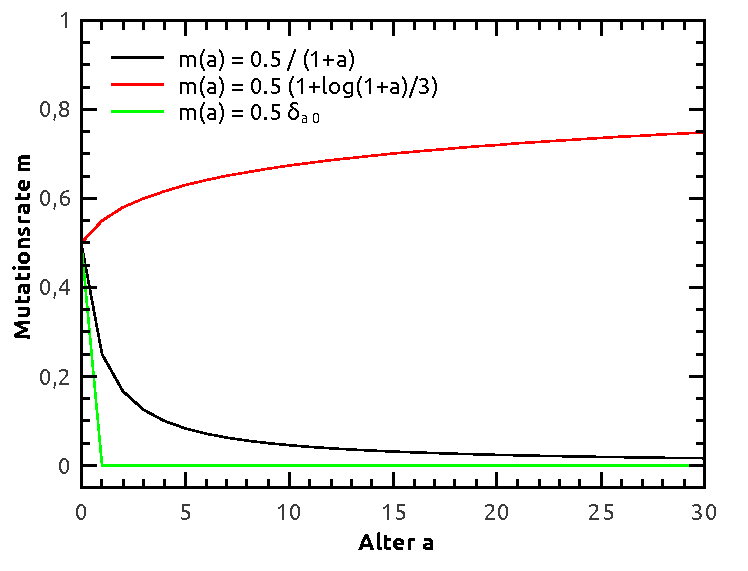
\includegraphics[width=10cm]{abbildungen/mutationsrate.pdf}
    
\end{frame}


% Framebeginn...%
\begin{frame}[t]\frametitle{Statistische Auswertung} 

	\only<1-2> {
		\textbf{Problem:}\\[-0.4cm]

		\begin{equation*}
			\left.
			\begin{array}{cl}
				(1) & \text{Initialisierung der Anfangs-}\\
					& \text{population zuf�llig} \\[0.2cm]
				(2) & \text{Umwelt- und Elternselektion }\\
					& \text{in Teilen zufallsabh�ngig} \\[0.2cm]
				(3) & \text{Mutation zufallsabh�ngig} \\
			\end{array}
			\right\}\quad \parbox{4.cm}{\textbf{Minimum bei jeder\newline Berechnung anders} }
		\end{equation*}
	}

	\only<2> {
		\textbf{L�sung:}\\
		\vspace{-0.4cm}
		\begin{center}
			\begin{tabular}{c}
				\textbf{50-fache} Fitness-Berechnung: $\{m_1, ..., m_{50}\}$ \\[-0.2cm]
				\begin{rotate}{-90} $\Longrightarrow$ \end{rotate}\\[0.55cm]
				\begin{tabular}{r l}				
					\textbf {gemittelte Fitness} $\mathbf{m}$ &\hspace{-0.45cm} $\boldsymbol{=} \bar{\mathbf{m}} \boldsymbol{\pm} \boldsymbol{\sigma}_\mathbf{m}$ \\
					\textbf {beste Fitness} $\mathbf{m}$ &\hspace{-0.45cm} $\boldsymbol{=} \boldsymbol{\min \{} \mathbf{m_1, ..., m_{50}} \boldsymbol{\}}$ 
				\end{tabular}
			\end{tabular}
		\end{center}
	}
\end{frame}

%%%%%%%%%%%%%%%%%%%%%%%%%%%%%%%%%%%%%%%%%%%%%
%	Ergebnisse konstante Mutationsrate		%
%%%%%%%%%%%%%%%%%%%%%%%%%%%%%%%%%%%%%%%%%%%%%

\section{Ergebnisse konstante Mutationsrate} 

\begin{frame}
    \begin{center}
	\LARGE{Konstante Mutationsrate}
    \end{center}
\end{frame}

\begin{frame}\frametitle{Optimale Fitnesswerte f�r $n = 2$} 

\end{frame}

\begin{frame}\frametitle{Mittlere Generationenanzahl bis Abbruch f�r $n = 2$} 

\end{frame}

%%%%%%%%%%%%%%%%%%%%%%%%%%%%%%%%%%%%%%%%%%%%%%%%%%%
%    Ergebnisse altersabh�ngige Mutationsrate     %
%%%%%%%%%%%%%%%%%%%%%%%%%%%%%%%%%%%%%%%%%%%%%%%%%%%

\section{Ergebnisse altersabh�ngige Mutationsrate}

\begin{frame}
    
    \begin{center}
	\LARGE{Altersabh�ngige Mutationsrate}
    \end{center}

\end{frame}

% Framebeginn...%
\begin{frame}\frametitle{Elternselektion detailiert} 

\end{frame}

\begin{frame}\frametitle{Mittleres Minimum f�r $n = 2$} 

\end{frame}

\begin{frame}\frametitle{Mittlere Generationenanzahl bis Abbruch f�r $n = 2$} 

\end{frame}

% Framebeginn...%
\begin{frame}\frametitle{Zusammenfassung}

\end{frame}

\end{document}

